\documentclass[../main.tex]{subfiles}

\begin{document}
\section{Results}\label{sec:results}
\subsection{Franke's function}

\subsubsection{OLS regression}
\subsubsection{The bias-variance tradeoff}
With a dataset of values produced from Franke's function (number of datapoints $N=18$, with random normally distributed noise added), we've fitted a model based on the training set and predicted new data based on the testing set. This was done with a design matrix of increasing degrees, from $1$ to $9$. The following figure \ref{fig:result_complexity} is a plot relating the mean squared error of the model to the complexity (or degree).

\begin{figure}[h]
    \centering
    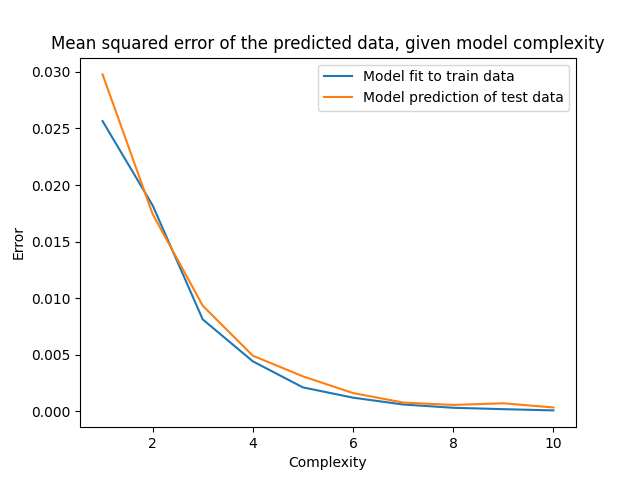
\includegraphics[width=\textwidth]{../assets/complexity.png}
    \caption{The error of a model based on the train and test set respectively, in relation to the polynomial degree of the model.}
    \label{fig:result_complexity}
\end{figure}

Once again, we produce a dataset from the Franke function (number of datapoints $N=40$, no noise added) and fit the model to design matrices of varying degree, from 1 to 15. Using The Bootstrap, we record the bias and variance (as they are explained in section \ref{sec:bv_decomp}. Figure \ref{fig:result_bias_variance} shows their relation with increasing complexity/degree of polynomial. 

\begin{figure}[h]
    \centering
    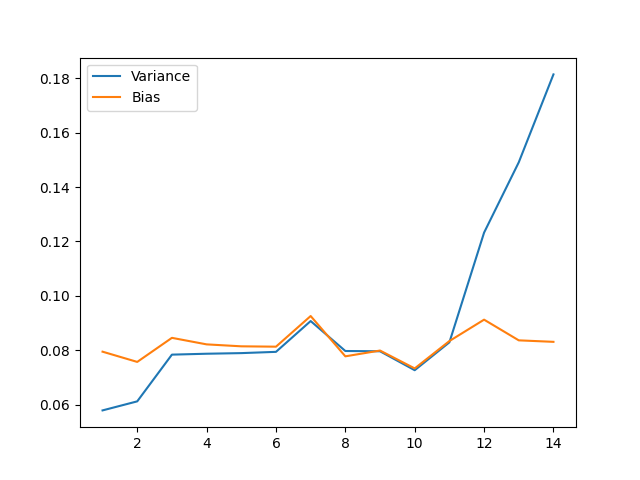
\includegraphics[width=\textwidth]{../assets/var.png}
    \label{fig:result_bias_variance}
    \caption{Bias and variance plotted in relation to the polynomial degree of the model.}
\end{figure}

The above results uses bootstrapping as an assessment technique. We have also implemented $K$-fold cross-validation, and figure \ref{fig:result_cv_boot_mse} shows how their calculated MSE compares

\begin{figure}[h]
    \centering
    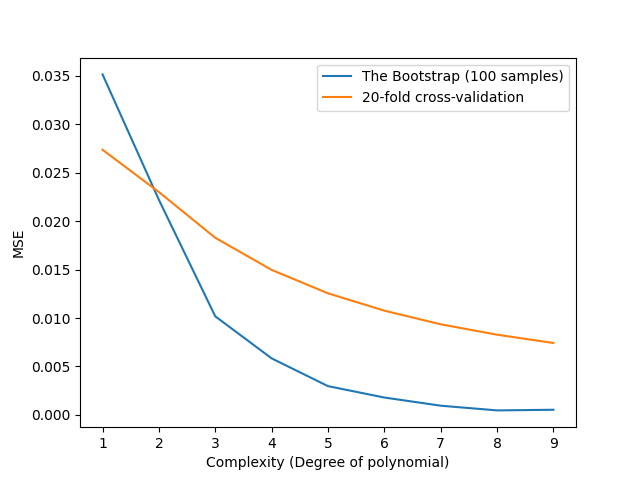
\includegraphics[width=\textwidth]{../assets/cv_boot_mse.png}
    \caption{Mean squared error calculated with $K=20$-fold cross-validation and bootstrapping with $B=100$.}
    \label{fig:result_cv_boot_mse}
\end{figure}

\subsubsection{Ridge regression}
\subsubsection{Lasso regression}

\subsection{Terrain data}
\begin{figure}[htb] 
   \centering
   \begin{subfigure}[b]{0.45\textwidth}
    \centering
    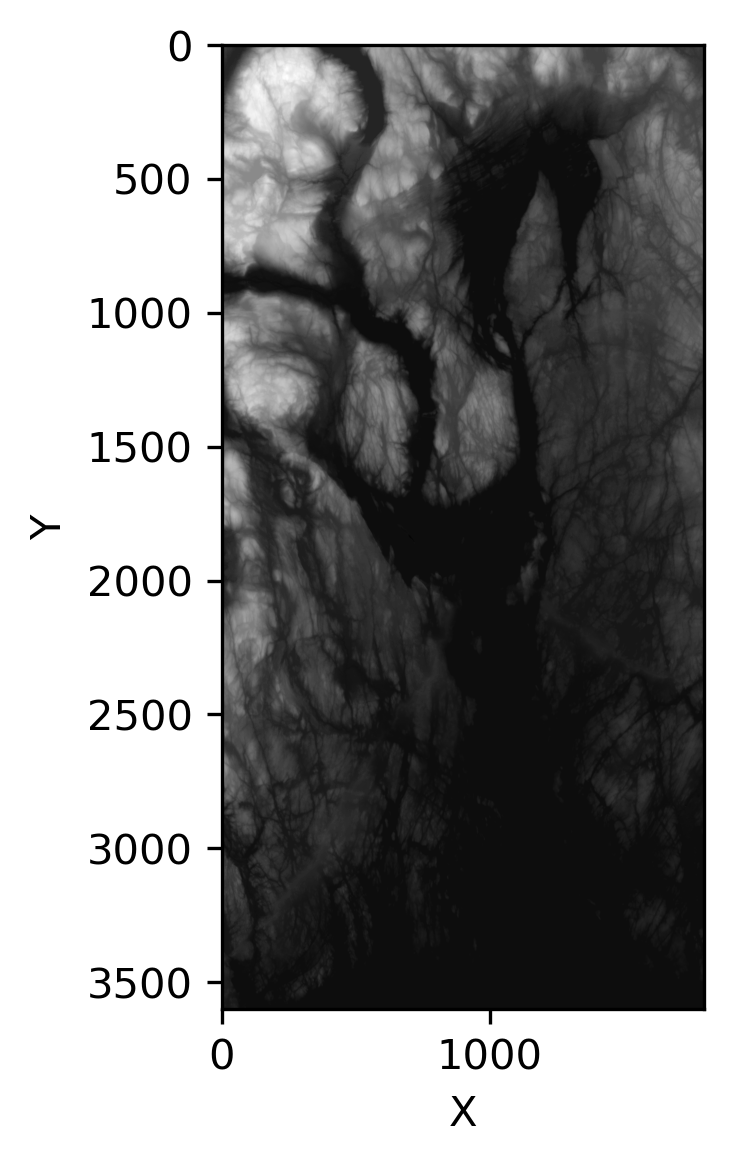
\includegraphics[width=\textwidth]{../assets/terrain_n59_e010.png} 
    \caption{}
    \label{fig:terrain_Norway}
   \end{subfigure}
   \quad
   \begin{subfigure}[b]{0.45\textwidth}
    \centering
    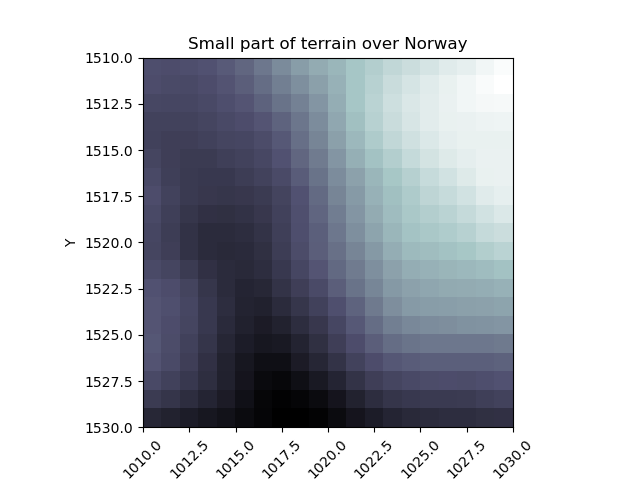
\includegraphics[width=\textwidth]{../assets/part_of_terrain.png} 
    \caption{}
   \end{subfigure}
   \caption{(a) Terrain data over Norway 59\degree north, 10\degree east. (b) Small part of the terrain data.}
\end{figure} 

\subsubsection{OLS}
\begin{figure}[htb] 
   \centering
   \begin{subfigure}[b]{0.45\textwidth}
    \centering
    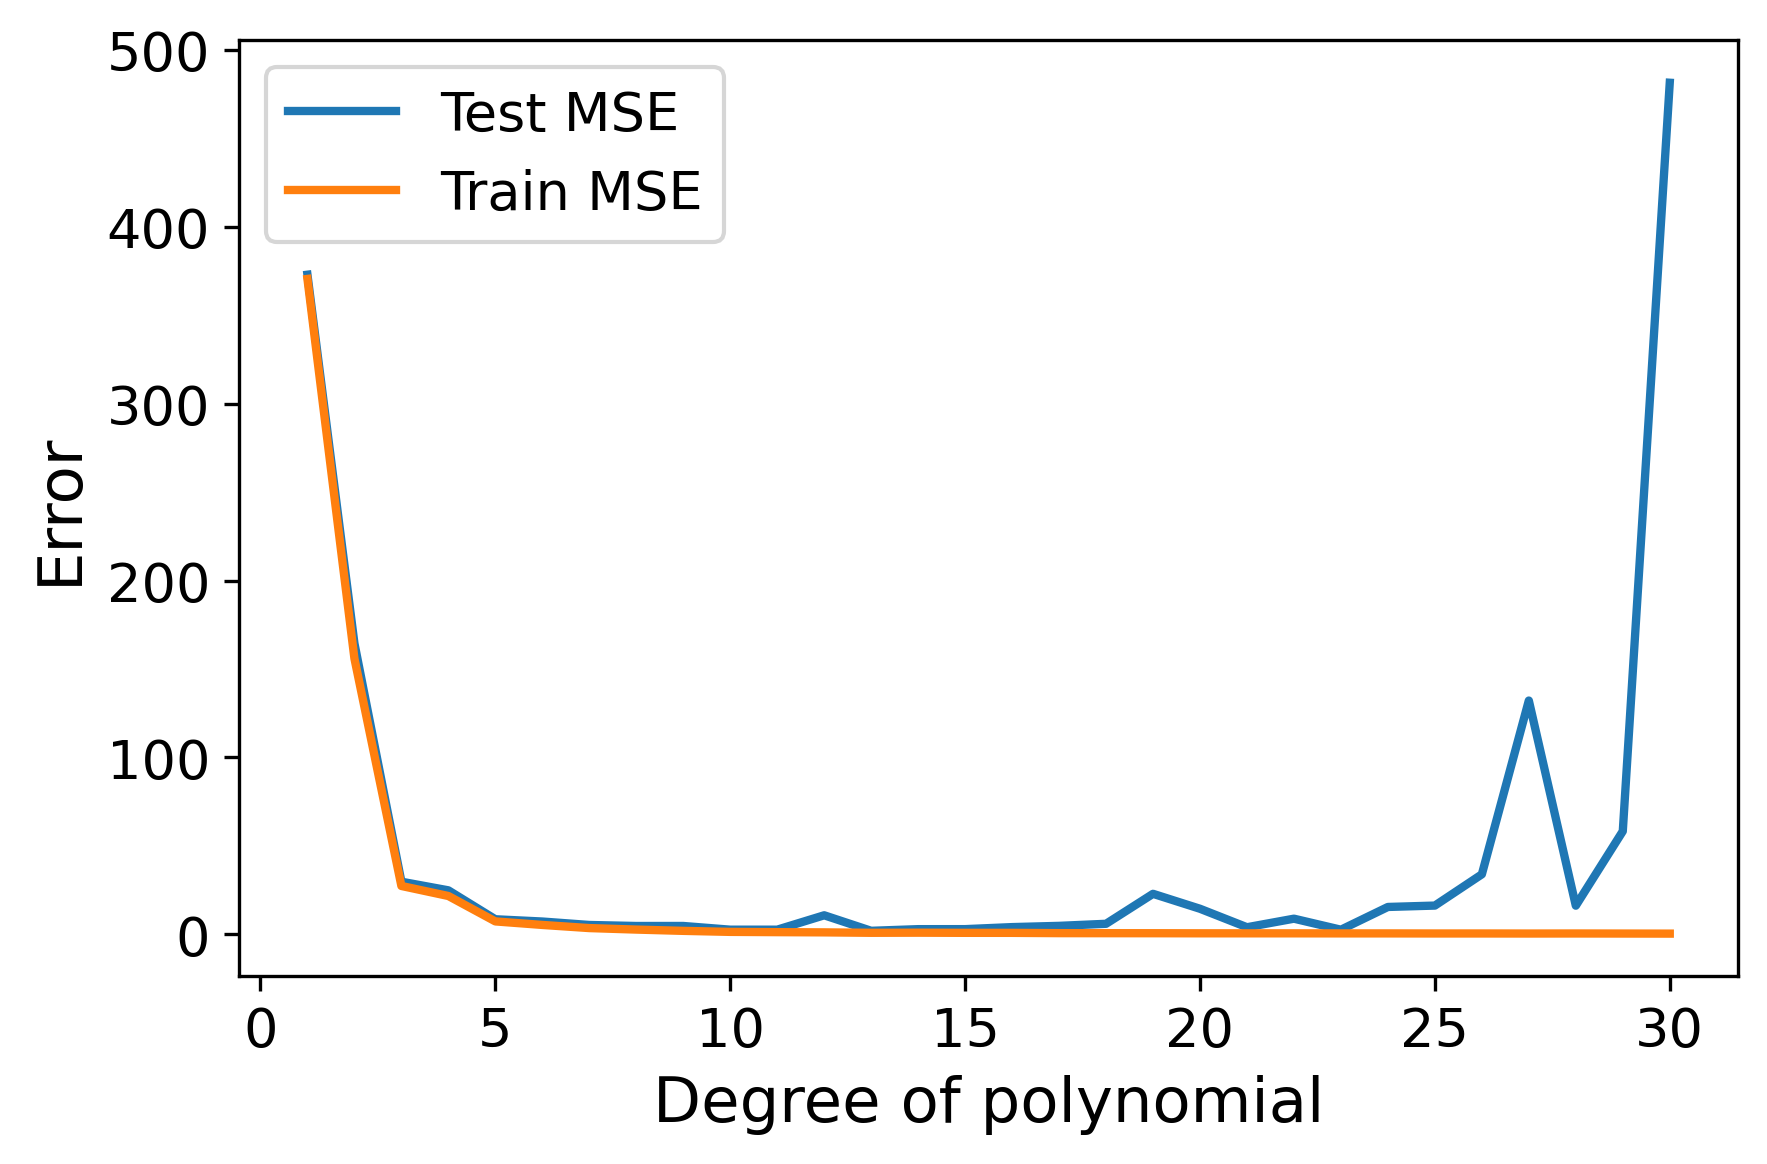
\includegraphics[width=\textwidth]{../assets/terrain_ols_error_plot.png} 
    \caption{}
    
   \end{subfigure}
   \quad
   \begin{subfigure}[b]{0.45\textwidth}
    \centering
    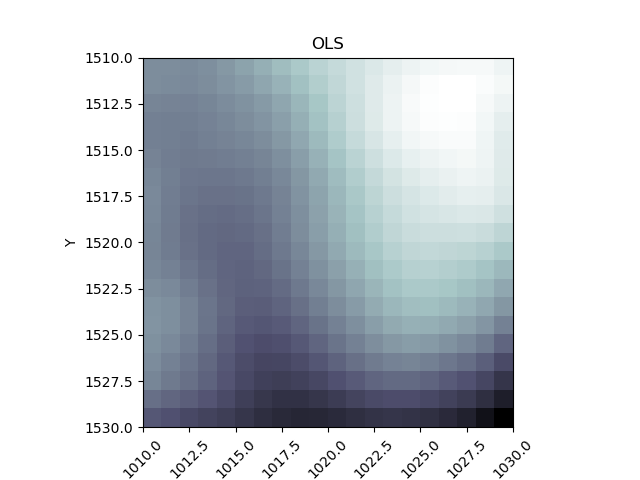
\includegraphics[width=\textwidth]{../assets/Terrain_OLS_bestdegree.png} 
    \caption{}
   \end{subfigure}
   \caption{(a) (b) 
   }
   \label{fig:terrain-OLS}
\end{figure} 


\subsubsection{Ridge regression}

\begin{figure}[htb] 
   \centering
   \begin{subfigure}[b]{0.45\textwidth}
    \centering
    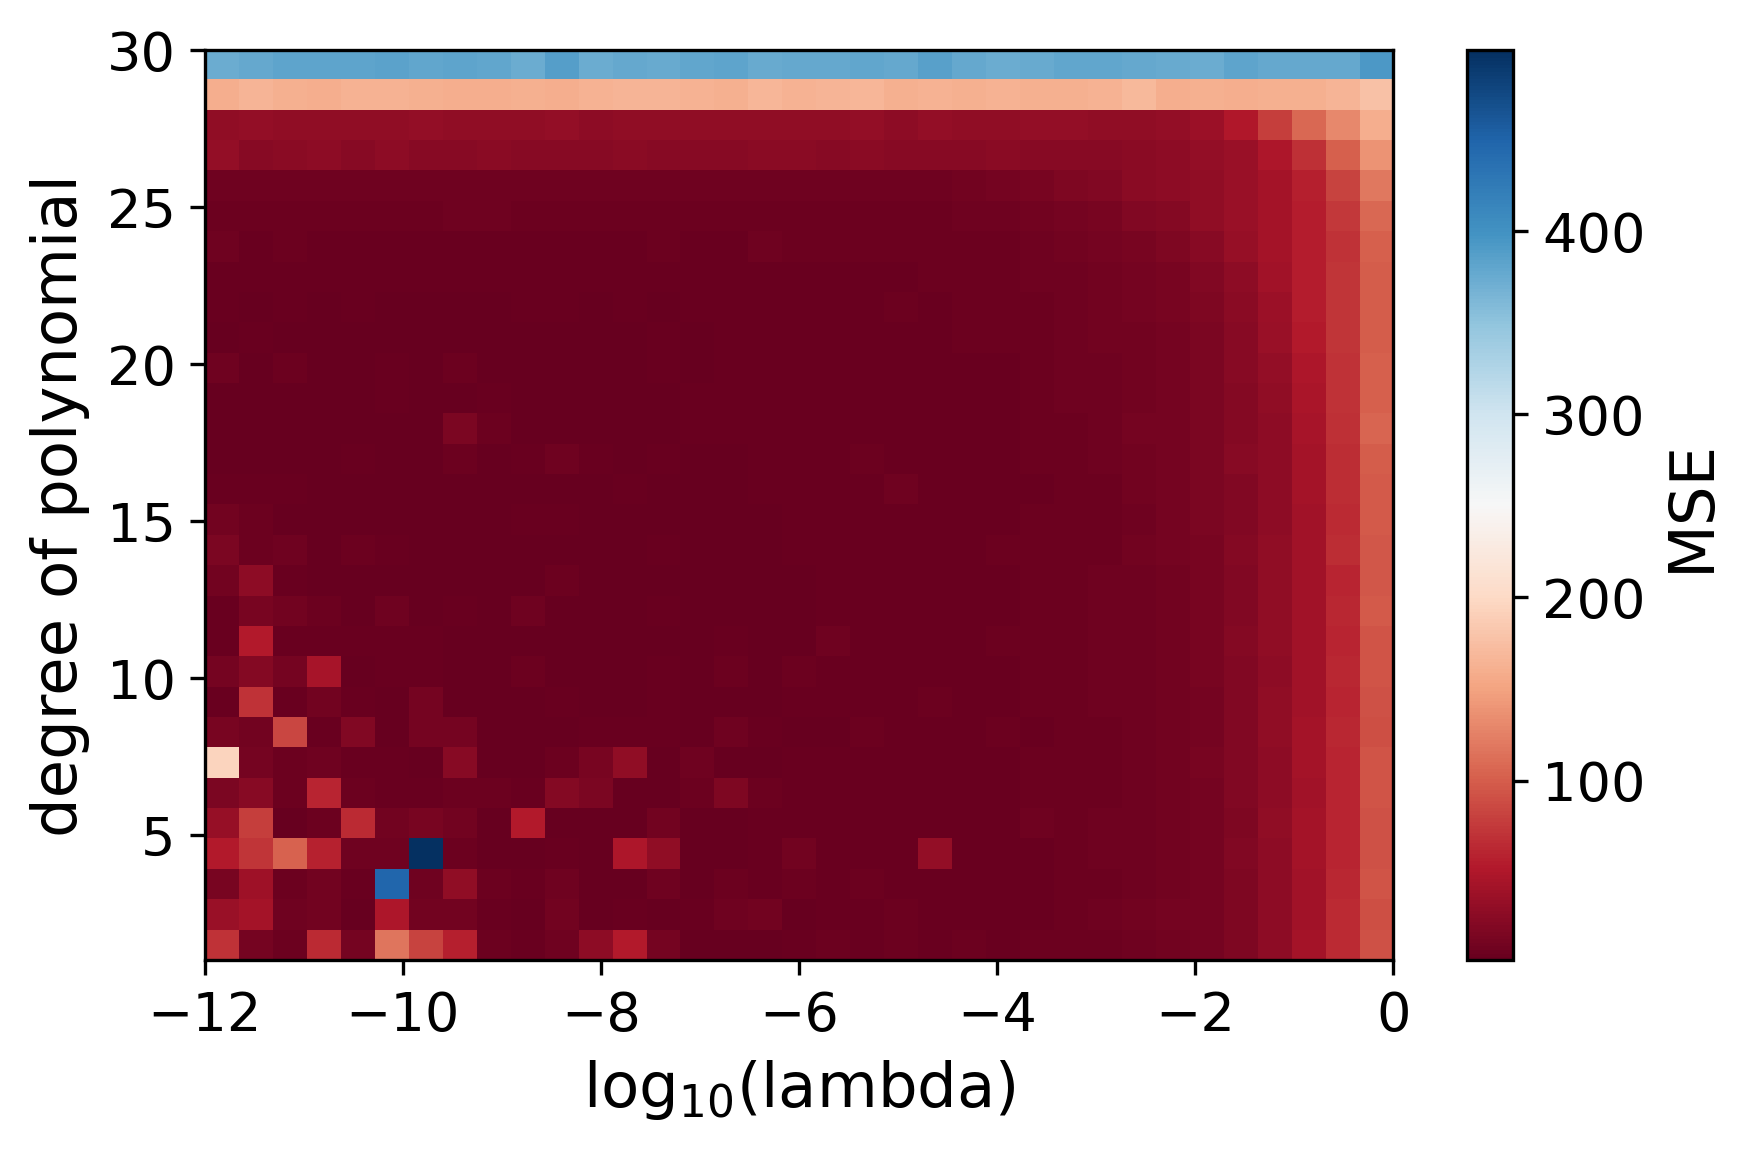
\includegraphics[width=\textwidth]{../assets/terrain-ridge-degree-lambda-colormap.png} 
    \caption{}
    
   \end{subfigure}
   \quad
   \begin{subfigure}[b]{0.45\textwidth}
    \centering
    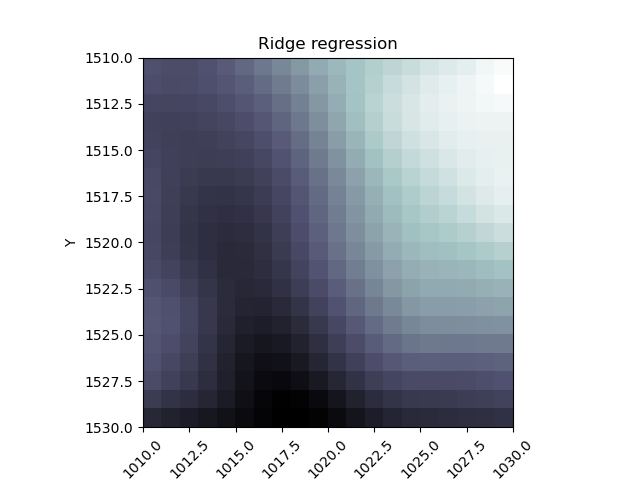
\includegraphics[width=\textwidth]{../assets/Terrain_ridge_bestdegree.png} 
    \caption{}
   \end{subfigure}
   \caption{(a) (b) 
   }
   \label{fig:terrain-ridge}
\end{figure} 

\subsubsection{Lasso regression}

\begin{figure}[htb] 
   \centering
   \begin{subfigure}[b]{0.45\textwidth}
    \centering
    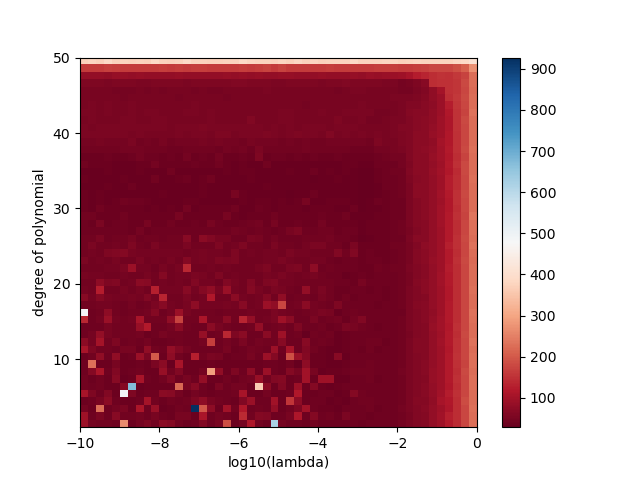
\includegraphics[width=\textwidth]{../assets/terrain-lasso-degree-lambda-colormap.png} 
    \caption{}
    
   \end{subfigure}
   \quad
   \begin{subfigure}[b]{0.45\textwidth}
    \centering
    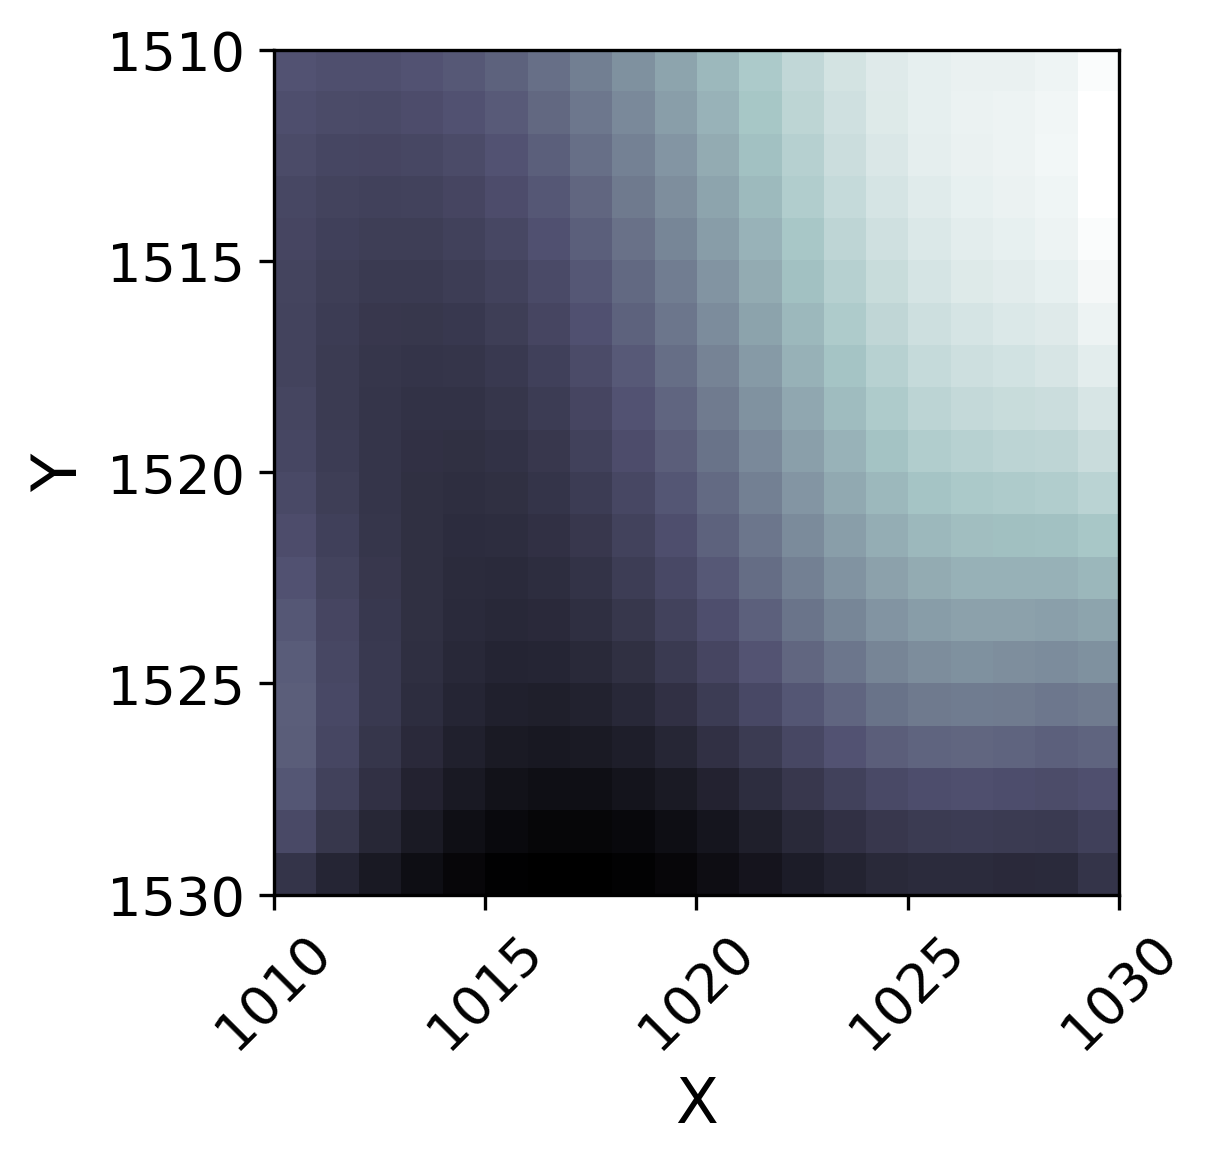
\includegraphics[width=\textwidth]{../assets/Terrain_lasso_bestdegree.png} 
    \caption{}
   \end{subfigure}
   \caption{(a) (b) 
   }
   \label{fig:terrain-lasso}
\end{figure} 

\end{document}
